\documentclass{sig-alternate}

\usepackage{enumitem}
\usepackage{framed}
\usepackage{listings}
\usepackage{amstext}
\usepackage{amstext}
\usepackage{pdfpages}
\usepackage{alltt}
\usepackage{epstopdf}
\usepackage{xspace,colortbl}
\usepackage[USenglish]{babel}
\usepackage{multirow}
\usepackage{url}
\usepackage{subfigure}
\usepackage{graphicx}
\usepackage{amssymb}
\usepackage{fmtcount}
\usepackage{amsfonts}
\usepackage{xspace}
\usepackage{amsmath}
\usepackage{multirow}
\usepackage[mathscr]{eucal}
%\usepackage{psfrag}
\usepackage{colortbl}
\usepackage{bm}
\usepackage[nospace]{cite}


\usepackage[algoruled,vlined,linesnumbered]{algorithm2e}
\usepackage{xcolor}
\newcommand\mycommfont[1]{\scriptsize\ttfamily\textcolor{blue}{#1}}
\SetCommentSty{mycommfont}
\SetKwFor{ParForAll}{for}{do in parallel}{end}
\SetKw{WaitUntil}{wait until}


\lstset{basicstyle=\scriptsize,breaklines=true}

\linespread{0.94}%

\makeatletter
\def\@copyrightspace{\relax}
\makeatother

\begin{document}

\setlength{\belowdisplayskip}{2pt} \setlength{\belowdisplayshortskip}{2pt}
\setlength{\abovedisplayskip}{2pt} \setlength{\abovedisplayshortskip}{2pt}
\setlength{\belowcaptionskip}{-8pt}
\selectfont

\newtheorem{theorem}{Theorem}
\newtheorem{example}{Example}
\newtheorem{definition}{Definition}
\newtheorem{proposition}{Proposition}
\newtheorem{lemma}{Lemma}
\newtheorem{corollary}{Corollary}

\newcommand{\cond}{\textrm{Cond}\xspace}
\newcommand{\dataset}{data set\xspace}
\newcommand{\datasets}{data sets\xspace}
\newcommand{\spview}{\textsf{SPView}\xspace}
\newcommand{\fjview}{\textsf{FJView}\xspace}
\newcommand{\aggview}{\textsf{AggView}\xspace}
\newcommand{\hashfunc}[1]{\textsf{hashfunc}(#1)\xspace}

\newcommand{\avgfunc}{\ensuremath{\texttt{avg} }\xspace}
\newcommand{\maxfunc}{\ensuremath{\texttt{max} }\xspace}
\newcommand{\minfunc}{\ensuremath{\texttt{min} }\xspace}
\newcommand{\histfunc}{\ensuremath{\texttt{histogram\_numeric} }\xspace}
\newcommand{\countfunc}{\ensuremath{\texttt{count}}\xspace}
\newcommand{\sumfunc}{\ensuremath{\texttt{sum} }\xspace}
\newcommand{\varfunc}{\ensuremath{\texttt{var} }\xspace}
\newcommand{\covfunc}{\ensuremath{\texttt{cov} }\xspace}
\newcommand{\corrfunc}{\ensuremath{\texttt{corr} }\xspace}
\newcommand{\medfunc}{\ensuremath{\texttt{median} }\xspace}
\newcommand{\percfunc}{\ensuremath{\texttt{percentile} }\xspace}
\newcommand{\havingfunc}{\ensuremath{\texttt{HAVING} }\xspace}
\newcommand{\ratio}{\ensuremath{\rho }\xspace}


\newcommand{\scp}{\textbf{SampleCleanPipeline}\xspace}
\newcommand{\sca}{\textbf{SampleCleanAlgorithm}\xspace}


\newcommand{\insertion}{\ensuremath{\texttt{INSERT} }\xspace}
\newcommand{\update}{\ensuremath{\texttt{UPDATE} }\xspace}
\newcommand{\delete}{\ensuremath{\texttt{DELETE} }\xspace}


\newcommand{\tbl}[1]{\textsf{#1}\xspace}
\newcommand{\field}[1]{\textsf{#1}\xspace}
\newcommand{\cost}{\textrm{cost}\xspace}
\newcommand{\ans}{\textsf{ans}\xspace}
\newcommand{\dans}{\Delta\textsf{ans}\xspace}
\newcommand{\cqp}{correction query processing\xspace}
\newcommand{\Cqp}{Correction query processing\xspace}

\newcommand{\reminder}[1]{{{\textcolor{magenta}{\{\{\bf #1\}\}}}\xspace}}
\newcommand{\specialcell}[2][c]{%
  \begin{tabular}[#1]{@{}c@{}}#2\end{tabular}}

\def\ojoin{\setbox0=\hbox{$\bowtie$}%
  \rule[-.02ex]{.25em}{.4pt}\llap{\rule[\ht0]{.25em}{.4pt}}}
\def\leftouterjoin{\mathbin{\ojoin\mkern-5.8mu\bowtie}}
\def\rightouterjoin{\mathbin{\bowtie\mkern-5.8mu\ojoin}}
\def\fullouterjoin{\mathbin{\ojoin\mkern-5.8mu\bowtie\mkern-5.8mu\ojoin}}

%\newcommand{\reminder}[1] {}
\pagestyle{plain}

\title{A Monte-Carlo Approach For Robust Execution of Heuristic Entity Resolution Pipelines}

\maketitle


\vspace{-1em}

\begin{abstract}
\reminder{TODO}
\end{abstract}


\section{Introduction}
Large datasets can be prone to error \cite{Gartner}, and data cleaning has been studied to mitigate query error on dirty data \cite{dasu2003exploratory, mayfield2010eracer, openrefine, wrangler, DBLP:conf/sigmod/DallachiesaEEEIOT13, DBLP:conf/pervasive/JefferyAFHW06}.
An important subclass of data cleaning problems are Entity Resolution (ER) problems which have had much research interest both historically and recently. \cite{DBLP:journals/pvldb/KopckeTR10, conf/dmkd/MongeE97, conf/sigmod/WhangMKTG09, conf/acl/FinkelM08, conf/sigmod/WangLF12, Fellegi1969, conf/sigmod/ArasuGK10, DBLP:journals/tkde/ElmagarmidIV07, journals/tkde/Christen11, getoor2005link}
In these problems, for every record we want to find a single canonical mapping between the record and a real-world entity.
This includes regularizing representations, removal of duplicate records, and removal of irrelevant records.

A popular theoretical model for ER is the functional dependency model.
The concept of a functional dependency has been well studied in the database literature 
and was proposed by Codd in 1974 \cite{codd1974recent}.
Recent work explores encoding ER primitives as types of functional dependencies called Conditional Functional Dependencies (CFD) \cite{bertossi2013data, fan2014interaction, fan2008conditional}.
These are basically rules that encode unsatisfied constraints based on expert input (i.e NY == New York) and the data cleaning algorithm iterates until these constraints are satisfied.
As this formulation fits nicely into a Satisfiability-like framework, many theoretical insights have naturally followed such determining the minimal sequence of data changes to satisfy all of the constraints is NP-Hard.

As the NP-Hard result suggests, while this model gives insights into what types of errors occur in a dataset, there is a challenge of efficiently repairing the errors (i.e. enforcing the constraints).
Bertossi et al. \cite{bertossi2013data} found that a lattice data structure could be used to a find PTIME iterative algorithm for ER problems with only ``matching" dependencies that fit certain cyclic conditions.
Wang et al. \cite{wang2014towards} extended the CFD framework with ``fixing" rules; rules that also prescribed fixes which as in Bertossi et al. makes the cleaning algorithms faster and more reliable.

A key assumption of the functional depedency work in data cleaning has been \emph{infallible} rules.
However, in practice, this is rarely the case.
Large datasets are often pre-processed with chains of heuristic data cleaning operations each with their own precision and recall characteristics as in ETL tools \cite{herzog2007data}.
Furthermore, increasingly data cleaning is part of a larger pipeline including streaming, machine learning, or exploratory data analysis.
In this setting, semantics on partial or sampled results are important, and the CFD model may not be appropriate to describe these applications.

In this work, we explore robust execution of \emph{pipelines} of data cleaning operations with an application to ER.
In contrast to prior work, we formalize ER as a composition of functions on relations as opposed to constraints on tuples in those relations.
We show that in the case where our operations are \emph{infallible}, our formalization naturally leads to the algorithm proposed by Bertossi et al., and exactly the same result with a connected components algorithm over a graph of linked tuples.
However, the connected components version is robust to transitivity errors in the rules which correspond to missing edges in the graph.
We introduce a data structure, which we call a \emph{proposal},  that propagates an augemnted intermediate state of the pipeline mitigating some types of errors.
We then devise an alternative to the connected components, accounting for spurious edges, using correlation clustering which seperates the graph into components that are approximately cliques.
Finally, we merge proposal data structures from different executions allowing us to try different permutations of the ER pipeline and take a consensus of their results.










\section{Background}

\subsection{Entity Resolution}
The entity resolution (ER) problem [cite] is the study of linking database records to real-world entities.
While traditionally, the operation only discusses the final step of duplicate record linkage [cite], there are often
many pre-processing steps such as string processing and imputation that are often run before record linkage.

We formalize this problem as a composition of two functional operations: deduplication and correction.
\begin{definition} Entity Resolution. 
An Entity Resolution task (ER) for a relation $R$ is a composition of the 
following deterministic operations:
\begin{itemize}
\item Correct $\kappa(R_i,a_{1})$ which for each record in $R_i$ returns a new record with attribute $a_{1}$ modified.
\item Deduplication $\delta(R_i)$ for each record in $R_i$ returns a new record such that the new record is contained in $R_i$.
\end{itemize}
%We constrain that $\kappa$ and $\delta$ are consistent; that is given two records that are identical on the projection their operation is identical.
\end{definition}

To make this more concrete, consider the following scenario. 
Suppose we want to count the number of Mediterranean restaurants in the city of Berkeley, and 
our dataset is of the following schema: \textbf{Restaurant(Name, Type, City)}.
This dataset contains duplicates (two records that point to the same real world entity) and missing type labels.
To fill in the missing type labels we can train a classifier on those labels that do exist and predict a label from the features of the restaurant name $\kappa$.
The operation that merges two records that refer to the same restaurant is a $\delta$ operation.

\subsection{Transitivity Errors Are Common When Using Heuristics}
Let us explore one type of error that can happen when $\delta$ and $\kappa$ are heuristics.
We can present a simplified problem to better understand the challenges.
A special case of the general ER problem posed above is ER on a string-valued single attribute.

The first problem is a false-negative problem.
We may find that string $a$ merges to string $b$, and $b$ merges to $c$. 
This would imply a linkage between $a$ and $c$; which is missing.
Our algorithmic challenge then is to find as many of these missing edges.
We argue that some of these edges can be discovered by making the graph more dense 
by also looking at the prior history of transformations that happened to the string (which we will discuss in the next section).

Conversely, another problem that can happen is spurious edges.
$a$ and $b$ are linked when in reality they are two separate entities.
In this case, the random permutations find and more highly weight those edges that are invariant to the permutation of operations.

\subsection{SampleCleanPipeline Basic API}
In SampleClean [cite], we proposed using sampling to scale data cleaning to large datasets.
Instead of cleaning an entire dataset, we applied an expensive data cleaning algorithm to a sample, then 
answer queries using the clean sample.
This allowed for previously prohibitively expensive techniques (eg. crowdsourcing) to still estimate results
on large datasets.

We implemented SampleClean as an application on the BDAS stack.
This application contains a library of data cleaning techniques, and an API to specify new data cleaning algorithms.
The main component of this library is the \scp class.
This class abstracts the management of execution of data cleaning operations away from the user.

Users define an ordered collection of data cleaning algorithms e.g. time format cleaning, nearest neighbor imputation, and Jaccard similarity deduplication.
Then, they define a series of hints of which constrain possible orders
of the data cleaning algorithms, e.g. run Algo1 before Algo2, run Algo2 last.
As in the examples, hints can be of the form of partial orders and absolute indices.

Once the pipeline is instantiated, there is an \textbf{optimize()} method which
translates the unordered collection and hints into an execution plan.
Then the \textbf{exec(sampleName)} method applies the pipeline to a sample.

\begin{lstlisting}
SampleCleanPipeline( 
  ops: Collection[SampleCleanAlgorithm],
  hints: List[Hints] 
) 


sample_clean_pipeline.optimize()

sample_clean_pipeline.exec("my_sample")
\end{lstlisting}

In this paper, we explore the final two steps, \textbf{optimize()} and \textbf{exec(sampleName)}, 
for a limited set of operators (ER operators).

The goal of SampleClean was to make data cleaning happen at interactive latencies. 
If EPS takes a long time to run this defeats the purpose of the system.
We also extend the API to the streaming case where partial results can stream back to the user.

\begin{lstlisting}
sample_clean_pipeline.stream_exec(
  "my_sample", 
  optimizer,
  onChangeCallback)
\end{lstlisting}

\subsubsection{Problem Statement}
We are given a collection of ER operators and hints that define partial orders and absolute indices.
The EPS algorithm has to output two things: (1) A data structure $T$ which represents an optimized plan (which call a \emph{proposal}), and
(2) translate $T$ into actual changes to the tuples in the sample.
For the streaming case, we define an incomplete optimization structure $T_k$ and an execution engine which updates its executions when the data
structure is updated $T_{k+1}\leftarrow T_k$. 












\section{Proposals}
We first look at subproblem relevant to the pipeline optimization; how do we represent the relationships 
between tuples in these entity resolution tasks.
We call this intermediate data structure a proposal since metaphorically the data cleaning operations propose changes.
The execution engine then takes this proposal and formulates an actionable execution plan based on the proposal actually apply the changes.

The solution will be to break apart the ER operators in the previous section and represent their operations
as a graph.
In this section, we describe this procedure for a single given pipeline.
Then, we discuss how to merge different proposals.

\subsection{Building Proposals}
We re-define entity resolution in terms of what we call \emph{proposal operations}.
That is instead of making a change, the operation proposes a candidate change.
By exposing this intermediate state rather than immediate applying changes, we can relax some of the assumptions we made
in the previous section when formalizing entity resolution.

First, $\delta$ operations need not execute one-to-one merges.
We can propose a set of candidate merges e.g. row1 one is linked to row2 and row3.
Similarly, with $\kappa$ operations we can propose a set of possible transformations e.g. if my attribute is a comma separated string value, the relevant data is either in 1st or 2nd field.
We can defer enforcing correctness to when the proposal is actually executed.
One way to think about this approach is that we are building a probabilistic database on a deterministic database and lazily marginalizing the distributions at execution time [cite].

\begin{definition} Entity Resolution Proposals. 
Proposal operations are functional operations on a weighted graph $G=(V,E,W(e),M(v))$ with edge weights $W(e)$ and a multiplicity function $M(v)$ for each vertex. 
Records in the database are represented as vertices, and proposed corrections/merges are represented as edges.
\begin{itemize}
\item Correct $\kappa(G,a_{1})$ For every $v \in V$, let $v'$ be the corrected version of $v$. We add $v'$ to $V$ if it does not exist and we draw an edge between $v$ and $v'$ with weight $w$ where a larger $w$ indicates increased confidence. If it already exists, we increment the multiplicty counter for $v'$. If $v$ has multiple possible corrected versions, repeat for all.
\item Deduplication $\delta(G)$ For every $v \in V$, draw an edge starting at $v$ to represent merging two records with weight $w$ where a larger $w$ indicates increased confidence. If it has multiple possible merges, draw edges for all.
\end{itemize}
%Like before, we constrain that $\kappa$ and $\delta$ are consistent; that is given two records that are identical on the projection their operation is identical.
\end{definition}

The end of a given pipeline will be a graph $G$. 
This graph structure is a generalization of the graph structure discussed in entity resolution [cite]; ie the graph in an open world model.

\subsection{Proposal API}
\reminder{TODO}

\subsection{Benefits from this Data Structure}
We list out some of the benefits of this data structure and what we can do with proposals that was not previously possible in pipeline of ``off-the-shelf" entity resolution components. First, proposals give a natural way to represent uncertainty using weighted edges. They also subsume deterministic algorithms as we can represent a tree of merges with uniform weights. It is true that internally, many ER algorithms use a similar construction, however, by building a single, unfied data structure to represent both $\kappa$ and $\delta$ operations, we can propagate the data structure through a pipeline of reusable components. 

The second benefit is a representation of history. 
By representing the $\kappa$ operations in the data structure, we do not lose history when we apply an operation.
For example, an operation might be correct for 80\% of records and give incorrect results for the last 20\%, and the data structure gives us a natural way to interface with previously correct results.

The practical implications of this structure are interesting. 
For example, in ER pipelines, we often have to make many decisions up front such as what string tokenizer to use, how to threshold heuristics, or how dates should be formatted.
In this model, with the proposal structure, we argue why not try all of them.
Obviously there is a tradeoff space between ER accuracy and performance, and we will discuss that more in the next section.

\subsection{Proposal Overhead}
The proposal framework introduces overhead as the graph $G$ is much larger in terms of both edges and vertices than typically considered in graph based ER tasks. 
This warrants new algorithms to process this larger graph.
If $p$ is the number of steps in the pipeline, and $k$ is the average number of candidates $O(p^2k^2+V^2)$.
\reminder{TODO}

\subsection{Algebra Over Proposals}
Given two different proposals $G_1$ and $G_2$, we can define a merge operations to make them a single proposal.
\reminder{TODO}


\section{Sampling and Ensembling Pipelines}
\reminder{TODO}
\subsection{Pipelines That Satisfy The Hints}
\reminder{TODO}
\subsection{Analysis of The Sampling}
\reminder{TODO}
\subsection{Prefix-based Optimized Execution}
\reminder{TODO}
%\section{Efficient Execution of Ensembled Pipelines}
\reminder{TODO}
\section{Streaming Progressive Correlation Clustering}
\reminder{TODO}
\section{Results}

\subsection{Does Randomization Make Pipelining More Robust?}
Compare to best single pipeline, worst single pipeline, and current state of the art.
We should find that a randomized execution is much better than the worst and hopefuly comparable to the best.
In some cases, it may be better than the best, but it should never be worse than the worst.

Dataset: MS Academic 
Operations: Filter and Deduplicate

Dataset: Yelp 
Operations: String Clean, City Format, Deduplicate

Dataset: Product 
Operations: identify sku if exists, string clean, Deduplicate

\begin{figure}[ht]
\centering
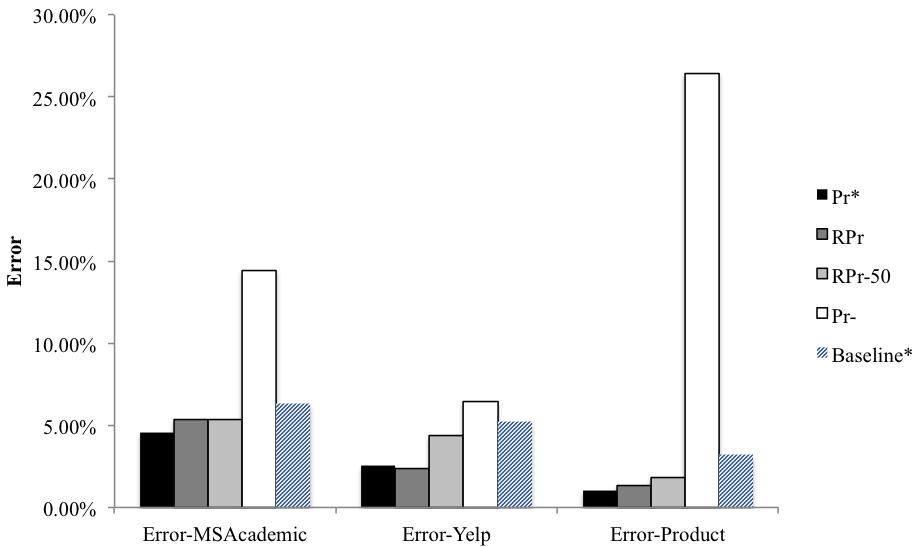
\includegraphics[scale=0.4]{fig1.png}
\caption{}
\label{exp:ms-academic-ranking}
\end{figure}

\subsection{How does this vary with random error in the operators?}
Should show that the more unreliable the data cleaning is the more that our approach benefits.

Introduce varying amount of random error (hashed so consistent between runs) into the ``city formatting" fix for the yelp dataset:

\begin{figure}[ht]
\centering
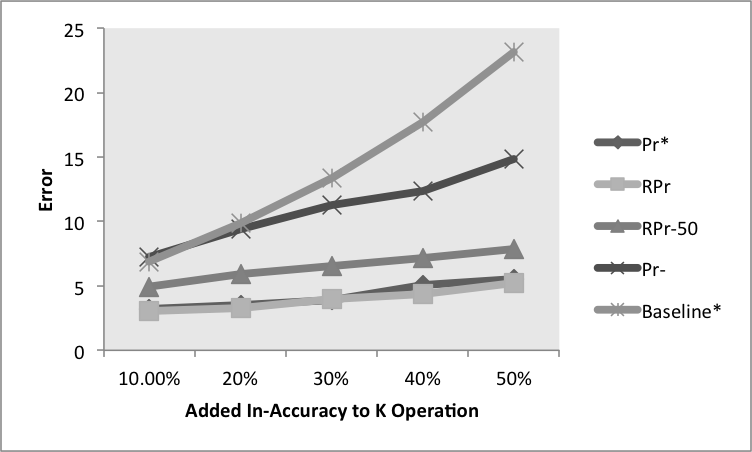
\includegraphics[scale=0.5]{fig2.png}
\caption{}
\label{exp:ms-academic-ranking}
\end{figure}

Introduce varying amound of random error (hashed so consistent between runs) into an extra dedup operation.

\begin{figure}[ht]
\centering
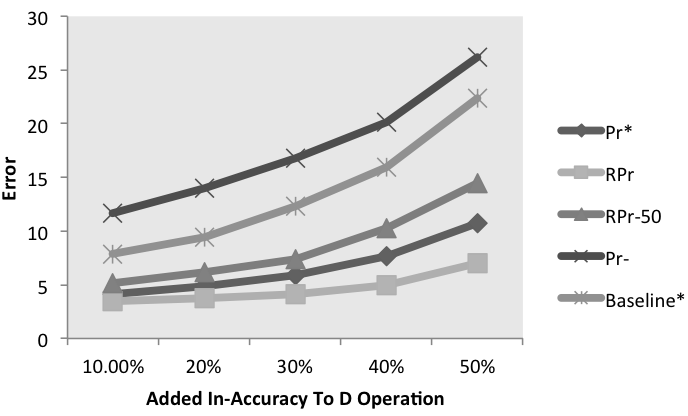
\includegraphics[scale=0.5]{fig3.png}
\caption{}
\label{exp:ms-academic-ranking}
\end{figure}

\subsection{Runtime-Accuracy Tradeoff}
Execute more samples and show how the accuracy improves.

\begin{figure}[ht]
\centering
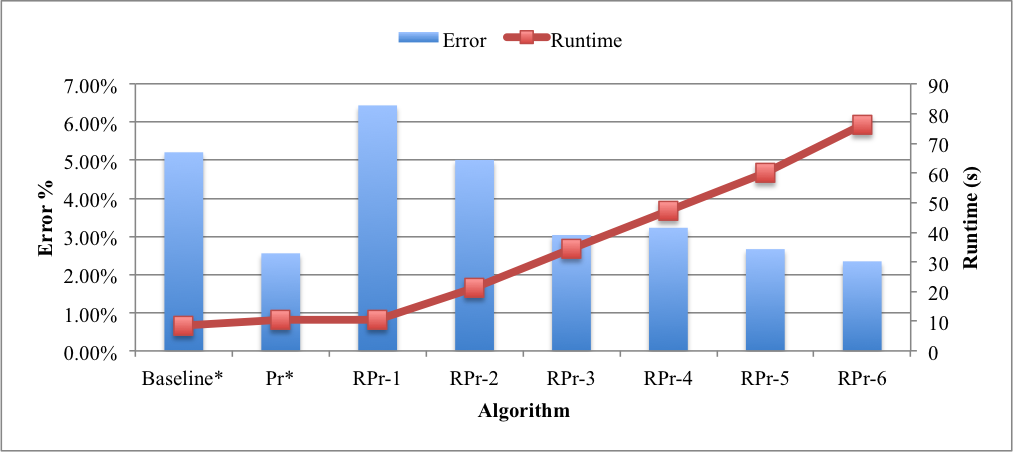
\includegraphics[scale=0.5]{fig4.png}
\caption{}
\label{exp:ms-academic-ranking}
\end{figure}


\subsection{Large-scale experiments}
Streaming correlation clustering. Show that at scale this technique can work and in a distributed environment.



\section{Conclusion}
\reminder{TODO}

\bibliographystyle{abbrv}
%\scriptsize
\fontsize{6.08pt}{6.4pt} \selectfont
\bibliographystyle{abbrv}
\bibliography{ref} 



\end{document}
